\documentclass[uplatex,dvipdfmx,11pt,a4paper]{jsarticle}
\usepackage[margin=20mm,headsep=7mm,footskip=12mm]{geometry}
\usepackage{amsmath,amssymb,mathtools,bm}
\usepackage{newtxtext,newtxmath}
\usepackage[haranoaji]{pxchfon}
\usepackage[dvipdfmx]{graphicx,xcolor}
\usepackage{tikz}
\usepackage[most]{tcolorbox}
\usepackage{fancyhdr}
\usepackage{enumitem}
\usepackage{tabularx,array,booktabs,multicol}
\usepackage{lastpage}
\usepackage{titlesec}
\usepackage{setspace}
\usepackage{ascmac}

\definecolor{Navy}{HTML}{17365D}
\definecolor{Blue}{HTML}{2F5597}
\definecolor{PaleBlue}{HTML}{EAF1F8}
\definecolor{Ink}{HTML}{202733}
\definecolor{SoftGray}{HTML}{F3F5F7}
\definecolor{RuleGray}{HTML}{D7DCE2}
\color{Ink}

\pagestyle{fancy}
\fancyhf{}
\fancyhead[L]{\small 基礎数学 予想模試 2026}
\fancyhead[R]{\small 電気通信大学大学院・基盤理工学専攻対策}
\fancyfoot[C]{\small \thepage\ / \pageref{LastPage}}
\renewcommand{\headrulewidth}{0.4pt}
\renewcommand{\footrulewidth}{0pt}

\setlength{\parindent}{1em}
\setlength{\parskip}{0.25em}
\setlist[enumerate,1]{label=(\arabic*),leftmargin=2.5em,itemsep=0.7em}
\setlist[enumerate,2]{label=(\alph*),leftmargin=2.5em,itemsep=0.5em}
\renewcommand{\arraystretch}{1.25}

\newtcolorbox{examinfo}[1][]{
  enhanced, colback=PaleBlue, colframe=Navy, boxrule=0.8pt,
  arc=1.5mm, left=3mm,right=3mm,top=2mm,bottom=2mm,#1}
\newtcolorbox{pointbox}[1][]{
  enhanced, colback=SoftGray, colframe=RuleGray, boxrule=0.5pt,
  arc=1mm, left=3mm,right=3mm,top=1.5mm,bottom=1.5mm,#1}
\newtcolorbox{solutionbox}[1][]{
  enhanced, breakable, colback=white, colframe=Navy, boxrule=0.7pt,
  arc=1mm, left=4mm,right=4mm,top=3mm,bottom=3mm,#1}
\newcommand{\score}[1]{\hfill\textcolor{Navy}{\fbox{\rule{0pt}{2.5ex}\,#1点\,}}}
\newcommand{\vect}[1]{\bm{#1}}
\newcommand{\R}{\mathbb{R}}
\newcommand{\dd}{\,\mathrm{d}}
\newcommand{\blanklines}[1]{%
\begin{tikzpicture}[x=1mm,y=1mm]
  \foreach \i in {0,...,#1}{\draw[RuleGray, line width=0.25pt] (0,-8*\i) -- (170,-8*\i);}
\end{tikzpicture}}

\begin{document}
% Cover
\thispagestyle{empty}
\begin{tikzpicture}[remember picture,overlay]
  \fill[Navy] (current page.north west) rectangle ([yshift=-62mm]current page.north east);
  \fill[Blue] ([yshift=-62mm]current page.north west) rectangle ([yshift=-66mm]current page.north east);
  \node[anchor=north,text=white,align=center] at ([yshift=-10mm]current page.north)
    {\Large 電気通信大学大学院};
  \node[anchor=north,text=white,align=center] at ([yshift=-20mm]current page.north)
    {\large 基盤理工学専攻 一般入試対策};
  \node[anchor=north,text=white,align=center] at ([yshift=-33mm]current page.north)
    {\fontsize{28}{34}\selectfont\bfseries 基礎数学 予想模試};
  \node[anchor=north,text=white,align=center] at ([yshift=-51mm]current page.north)
    {\Large 2026年度実施試験 対応};
\end{tikzpicture}

\vspace*{62mm}
\begin{center}
\begin{minipage}{0.82\textwidth}
\begin{examinfo}
\centering
\begin{tabular}{>{\bfseries}rl}
推奨時間 & 45分 \\
満点 & 100点 \\
構成 & 線形代数・多変数解析・重積分・微分方程式 \\
難易度 & 本試験標準 - やや難 \\
\end{tabular}
\end{examinfo}
\end{minipage}
\end{center}

\vfill
\begin{center}
\begin{minipage}{0.82\textwidth}
\small
本冊子は、2019--2025年度の出題傾向を踏まえて作成したオリジナル模試である。近年の頻出分野である固有値・固有空間を軸に、出題間隔を考慮して変数変換による重積分と常微分方程式を組み合わせた。
\end{minipage}
\end{center}
\vspace{12mm}
\begin{flushright}
氏名：\rule{55mm}{0.4pt}\qquad 得点：\rule{20mm}{0.4pt} / 100
\end{flushright}
\newpage

% Instructions
\section*{受験上の注意}
\begin{examinfo}
\begin{enumerate}
  \item 制限時間は45分を目安とする。
  \item 電卓・参考書は使用しない。
  \item 結果だけでなく、主要な計算過程を記すこと。
  \item 行列の固有空間では、基底を列ベクトルで明示すること。
  \item 重積分では、変数変換・領域・ヤコビアンを必ず示すこと。
  \item 微分方程式では、一般解を求めた後に初期条件を適用すること。
\end{enumerate}
\end{examinfo}

\vspace{5mm}
\section*{配点と時間配分の目安}
\begin{center}
\begin{tabularx}{0.92\textwidth}{c X c c}
\toprule
大問 & 主題 & 配点 & 目安時間 \\
\midrule
1 & 固有値・固有空間・対角化・行列のべき & 40点 & 18分 \\
2 & 極値判定・変数変換による重積分 & 35点 & 16分 \\
3 & 1階・2階常微分方程式 & 25点 & 11分 \\
\bottomrule
\end{tabularx}
\end{center}

\vspace{6mm}
\begin{pointbox}
\textbf{得点目標}
\quad 80点以上：非常に良い \quad 65--79点：合格圏 \quad 50--64点：要復習 \quad 49点以下：基礎事項を再確認
\end{pointbox}

\vfill
\begin{center}
\Large\bfseries 問題は次ページから
\end{center}
\newpage

% Problem 1
\section*{第1問　線形代数 \score{40}}
実数パラメータ $a$ に対して、行列
\[
A=\begin{pmatrix}
1 & a & 0\\
0 & 1 & 0\\
1 & 0 & 2
\end{pmatrix}
\]
を考える。以下の問いに答えよ。

\begin{enumerate}
  \item 特性多項式 $\det(\lambda I-A)$ を求め、$A$ の固有値をすべて求めよ。\score{8}
  \item 固有値 $\lambda=1$ および $\lambda=2$ に対する固有空間の基底を、$a=0$ と $a\neq 0$ の場合に注意して求めよ。\score{10}
  \item $A$ が対角化可能となるための $a$ の条件を求めよ。\score{6}
  \item 以下では $a=0$ とする。可逆行列 $P$ と対角行列 $D$ を一組求め、
  \[
  A=PDP^{-1}
  \]
  と表せ。\score{8}
  \item 自然数 $n$ に対して $A^n$ を求めよ。\score{8}
\end{enumerate}

\vfill
\begin{pointbox}
\textbf{答案上の注意：} 固有値の代数的重複度と固有空間の次元を区別して記述すること。
\end{pointbox}
\newpage

% Problem 2
\section*{第2問　多変数解析・重積分 \score{35}}
\begin{enumerate}
  \item 2変数関数
  \[
  f(x,y)=x^3+y^3-3xy
  \]
  について、停留点をすべて求め、それぞれが極大点・極小点・鞍点のいずれであるか判定せよ。必要に応じてヘッセ行列を用いてよい。\score{15}

  \item 領域
  \[
  D=\left\{(x,y)\in\R^2\mid 1\le x+y\le 2,\quad 0\le x-y\le 1\right\}
  \]
  に対して、重積分
  \[
  I=\iint_D (x^2-y^2)e^{x+y}\dd x\dd y
  \]
  を求めよ。変数変換
  \[
  u=x+y,\qquad v=x-y
  \]
  を用いてよい。\score{20}
\end{enumerate}

\vspace{6mm}
\begin{center}
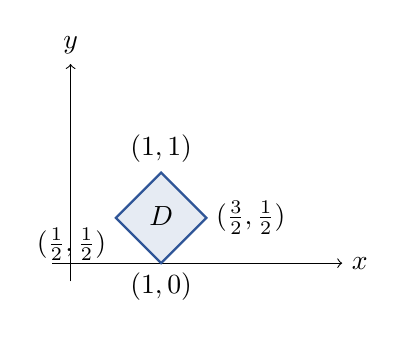
\begin{tikzpicture}[scale=1.15]
  \draw[->] (-0.2,0) -- (3.0,0) node[right] {$x$};
  \draw[->] (0,-0.2) -- (0,2.2) node[above] {$y$};
  \fill[Blue!12] (0.5,0.5)--(1,0)--(1.5,0.5)--(1,1)--cycle;
  \draw[Blue,thick] (0.5,0.5)--(1,0)--(1.5,0.5)--(1,1)--cycle;
  \node[below left] at (0.5,0.5) {$(\frac12,\frac12)$};
  \node[below] at (1,0) {$(1,0)$};
  \node[right] at (1.5,0.5) {$(\frac32,\frac12)$};
  \node[above] at (1,1) {$(1,1)$};
  \node at (1,0.52) {$D$};
\end{tikzpicture}
\end{center}
\newpage

% Problem 3
\section*{第3問　常微分方程式 \score{25}}
以下の初期値問題を解け。

\begin{enumerate}
  \item
  \[
  y'+2xy=x,\qquad y(0)=0.
  \]
  \score{10}

  \item
  \[
  y''-2y'+y=e^x,\qquad y(0)=0,\quad y'(0)=1.
  \]
  \score{15}
\end{enumerate}

\vspace{10mm}
\begin{pointbox}
\textbf{確認事項：}
1階方程式では積分因子を明示すること。2階方程式では右辺 $e^x$ が同次方程式の解と重なることに注意すること。
\end{pointbox}

\vfill
\begin{center}
\large\bfseries ここまでが問題編です。続いて解答用紙があります。
\end{center}
\newpage

% Answer sheets
\thispagestyle{fancy}
\section*{解答用紙 1　　第1問}
\begin{flushright}
氏名：\rule{45mm}{0.4pt}\qquad 得点：\rule{15mm}{0.4pt} / 40
\end{flushright}
\blanklines{28}
\newpage

\section*{解答用紙 2　　第2問}
\begin{flushright}
氏名：\rule{45mm}{0.4pt}\qquad 得点：\rule{15mm}{0.4pt} / 35
\end{flushright}
\blanklines{28}
\newpage

\section*{解答用紙 3　　第3問}
\begin{flushright}
氏名：\rule{45mm}{0.4pt}\qquad 得点：\rule{15mm}{0.4pt} / 25
\end{flushright}
\blanklines{28}
\newpage

% Solutions separator
\thispagestyle{empty}
\begin{tikzpicture}[remember picture,overlay]
  \fill[Navy] (current page.south west) rectangle (current page.north east);
\end{tikzpicture}
\vspace*{55mm}
\begin{center}
{\color{white}
{\fontsize{30}{36}\selectfont\bfseries 解答・採点基準\par}
\vspace{8mm}
{\Large 基礎数学 予想模試 2026\par}
\vspace{18mm}
{\large 採点後は、誤答の原因を「知識不足」「計算ミス」「時間不足」に分類すること。\par}
}
\end{center}
\newpage

% Solution 1
\section*{第1問　解答・採点基準 \score{40}}
\begin{solutionbox}
\textbf{(1) 特性多項式と固有値}\hfill【8点】

\[
\lambda I-A=
\begin{pmatrix}
\lambda-1 & -a & 0\\
0 & \lambda-1 & 0\\
-1 & 0 & \lambda-2
\end{pmatrix}.
\]
第2行または第3列に着目すると、
\[
\det(\lambda I-A)=(\lambda-1)^2(\lambda-2).
\]
したがって、固有値は
\[
\boxed{\lambda=1\ \text{（代数的重複度2）},\qquad \lambda=2\ \text{（代数的重複度1）}}.
\]

\textbf{配点：} 特性多項式5点、固有値と重複度3点。
\end{solutionbox}

\begin{solutionbox}
\textbf{(2) 固有空間}\hfill【10点】

$\lambda=1$ のとき、$\vect{x}=(x,y,z)^{\mathsf T}$ とすると
\[
(A-I)\vect{x}=
\begin{pmatrix}
0&a&0\\
0&0&0\\
1&0&1
\end{pmatrix}
\begin{pmatrix}x\\y\\z\end{pmatrix}=\vect{0}
\]
より
\[
ay=0,\qquad x+z=0.
\]
よって、
\[
E_1=\begin{cases}
\operatorname{span}\left\{
\begin{pmatrix}-1\\0\\1\end{pmatrix},
\begin{pmatrix}0\\1\\0\end{pmatrix}
\right\}, & a=0,\\[5mm]
\operatorname{span}\left\{
\begin{pmatrix}-1\\0\\1\end{pmatrix}
\right\}, & a\neq 0.
\end{cases}
\]

$\lambda=2$ のとき、
\[
(A-2I)\vect{x}=\vect{0}
\]
から $x=0,\ y=0$、$z$ は自由である。したがって
\[
\boxed{E_2=\operatorname{span}\left\{\begin{pmatrix}0\\0\\1\end{pmatrix}\right\}}.
\]

\textbf{配点：} $E_1$ の場合分け6点、$E_2$ 4点。
\end{solutionbox}

\newpage
\begin{solutionbox}
\textbf{(3) 対角化可能条件}\hfill【6点】

$\lambda=1$ の代数的重複度は2である。対角化可能であるためには、その固有空間の次元も2でなければならない。

$a=0$ では $\dim E_1=2$、$\dim E_2=1$ であり、一次独立な固有ベクトルが合計3本得られる。一方、$a\neq0$ では $\dim E_1=1$ で、合計2本しか得られない。
\[
\boxed{A\text{ が対角化可能 }\Longleftrightarrow a=0.}
\]
\end{solutionbox}

\begin{solutionbox}
\textbf{(4) 対角化}\hfill【8点】

$a=0$ とする。固有ベクトルを列に並べて
\[
P=\begin{pmatrix}
-1&0&0\\
0&1&0\\
1&0&1
\end{pmatrix},
\qquad
D=\begin{pmatrix}
1&0&0\\
0&1&0\\
0&0&2
\end{pmatrix}
\]
とおけば、$\det P=-1\neq0$ であり、
\[
AP=PD
\]
が成り立つ。したがって
\[
\boxed{A=PDP^{-1}}.
\]
この $P$ については $P^{-1}=P$ である。
\end{solutionbox}

\begin{solutionbox}
\textbf{(5) $A^n$}\hfill【8点】

対角化を用いると
\[
A^n=PD^nP^{-1},\qquad
D^n=\operatorname{diag}(1,1,2^n).
\]
よって
\[
\boxed{
A^n=\begin{pmatrix}
1&0&0\\
0&1&0\\
2^n-1&0&2^n
\end{pmatrix}}
\qquad (n=1,2,3,\ldots).
\]

\textbf{検算：} $n=1$ を代入すると元の行列 $A$ に一致する。
\end{solutionbox}

\begin{pointbox}
\textbf{第1問の典型的失点}
\begin{itemize}[leftmargin=2em,itemsep=0.2em]
\item $a\neq0$ でも $y$ を自由変数としてしまう。
\item 固有値が重複しているだけで「対角化不可能」と判断する。
\item $A^n$ で $2^n-1$ を $n2^{n-1}$ と誤る。
\end{itemize}
\end{pointbox}
\newpage

% Solution 2
\section*{第2問　解答・採点基準 \score{35}}
\begin{solutionbox}
\textbf{(1) 停留点と極値判定}\hfill【15点】

偏微分すると
\[
f_x=3x^2-3y,\qquad f_y=3y^2-3x.
\]
停留点では
\[
y=x^2,\qquad x=y^2.
\]
これらを合わせると $x=x^4$ であるから、実数解は $x=0,1$。したがって停留点は
\[
(0,0),\qquad (1,1)
\]
である。

ヘッセ行列は
\[
H_f(x,y)=\begin{pmatrix}
6x&-3\\
-3&6y
\end{pmatrix}.
\]

$(0,0)$ では
\[
\det H_f(0,0)=-9<0
\]
なので鞍点である。

$(1,1)$ では
\[
\det H_f(1,1)=36-9=27>0,\qquad f_{xx}(1,1)=6>0
\]
なので極小点である。極小値は
\[
f(1,1)=1+1-3=-1.
\]
よって
\[
\boxed{(0,0)\text{ は鞍点},\qquad (1,1)\text{ は極小点（極小値 }-1\text{）}}.
\]
極大点は存在しない。

\textbf{配点：} 停留点8点、ヘッセ行列と判定7点。
\end{solutionbox}

\begin{solutionbox}
\textbf{(2) 変数変換による重積分}\hfill【20点】

\[
u=x+y,\qquad v=x-y
\]
とおくと
\[
x=\frac{u+v}{2},\qquad y=\frac{u-v}{2}.
\]
ヤコビアンは
\[
\frac{\partial(x,y)}{\partial(u,v)}=
\begin{vmatrix}
\frac12&\frac12\\[1mm]
\frac12&-\frac12
\end{vmatrix}=-\frac12
\]
であるから
\[
\left|\frac{\partial(x,y)}{\partial(u,v)}\right|=\frac12.
\]
また、領域は
\[
1\le u\le2,\qquad 0\le v\le1
\]
という長方形に移る。さらに
\[
x^2-y^2=(x+y)(x-y)=uv.
\]
したがって
\begin{align*}
I&=\int_1^2\int_0^1 uv e^u\cdot\frac12\dd v\dd u\\
&=\frac12\left(\int_1^2u e^u\dd u\right)
\left(\int_0^1v\dd v\right)\\
&=\frac14\int_1^2u e^u\dd u.
\end{align*}
部分積分により
\[
\int u e^u\dd u=(u-1)e^u
\]
なので
\[
I=\frac14\left[(u-1)e^u\right]_1^2
=\boxed{\frac{e^2}{4}}.
\]

\textbf{配点：} 逆変換3点、領域4点、ヤコビアン5点、被積分関数の変換3点、積分計算5点。
\end{solutionbox}

\begin{pointbox}
\textbf{第2問の典型的失点}
\begin{itemize}[leftmargin=2em,itemsep=0.2em]
\item ヤコビアンの符号をそのまま使い、絶対値を取らない。
\item $x^2-y^2=(x+y)(x-y)$ に気付かず計算を複雑にする。
\item ヘッセ行列の行列式だけで極小・極大を判定し、$f_{xx}$ の符号を確認しない。
\end{itemize}
\end{pointbox}
\newpage

% Solution 3
\section*{第3問　解答・採点基準 \score{25}}
\begin{solutionbox}
\textbf{(1) 1階線形微分方程式}\hfill【10点】

\[
y'+2xy=x
\]
の積分因子は
\[
\mu(x)=\exp\left(\int 2x\dd x\right)=e^{x^2}
\]
である。両辺に $e^{x^2}$ を掛けると
\[
\frac{\dd}{\dd x}\left(e^{x^2}y\right)=xe^{x^2}.
\]
積分して
\[
e^{x^2}y=\frac12e^{x^2}+C
\]
より
\[
y=\frac12+Ce^{-x^2}.
\]
初期条件 $y(0)=0$ から $C=-\frac12$。したがって
\[
\boxed{y(x)=\frac12\left(1-e^{-x^2}\right)}.
\]

\textbf{配点：} 積分因子3点、一般解4点、初期条件3点。
\end{solutionbox}

\begin{solutionbox}
\textbf{(2) 2階非同次線形微分方程式}\hfill【15点】

同次方程式
\[
y''-2y'+y=0
\]
の特性方程式は
\[
r^2-2r+1=(r-1)^2=0
\]
であるから、同次解は
\[
y_h=(C_1+C_2x)e^x.
\]

右辺 $e^x$ は同次解と重なり、さらに $r=1$ は重解である。そこで
\[
y=e^xv(x)
\]
とおくと
\[
y''-2y'+y=e^xv''.
\]
したがって $v''=1$ であり、
\[
v=\frac{x^2}{2}+C_2x+C_1.
\]
よって一般解は
\[
y=e^x\left(\frac{x^2}{2}+C_2x+C_1\right).
\]
初期条件 $y(0)=0$ より $C_1=0$。また
\[
y'=e^x(v+v')
\]
であるため、$y'(0)=C_1+C_2=1$ より $C_2=1$。したがって
\[
\boxed{y(x)=e^x\left(x+\frac{x^2}{2}\right)}.
\]

\textbf{配点：} 同次解4点、共鳴への対応5点、一般解3点、初期条件3点。
\end{solutionbox}

\begin{pointbox}
\textbf{第3問の典型的失点}
\begin{itemize}[leftmargin=2em,itemsep=0.2em]
\item 1階方程式の積分因子を $e^{2x}$ とする。
\item 2階方程式で特殊解を $Ae^x$ と仮定し、同次解との重複を見落とす。
\item 初期条件を一般解に代入する前に微分計算を簡略化しすぎて符号を誤る。
\end{itemize}
\end{pointbox}
\newpage

% Review page
\section*{復習チェックリスト}
\begin{examinfo}
次回の演習までに、誤答した項目へチェックを入れて解き直すこと。
\end{examinfo}

\vspace{4mm}
\begin{tabularx}{\textwidth}{>{\centering\arraybackslash}p{8mm} X >{\centering\arraybackslash}p{24mm}}
\toprule
確認 & 到達目標 & 状態 \\
\midrule
$\square$ & 特性多項式を展開せず、三角形構造や零成分を利用して計算できる。 & 未 / 済 \\
$\square$ & 代数的重複度と幾何学的重複度を区別できる。 & 未 / 済 \\
$\square$ & 対角化 $A=PDP^{-1}$ から $A^n=PD^nP^{-1}$ を計算できる。 & 未 / 済 \\
$\square$ & 停留点を連立方程式として漏れなく求められる。 & 未 / 済 \\
$\square$ & ヘッセ行列による極値判定ができる。 & 未 / 済 \\
$\square$ & 変数変換後の領域とヤコビアンを正しく書ける。 & 未 / 済 \\
$\square$ & 1階線形微分方程式の積分因子を即座に作れる。 & 未 / 済 \\
$\square$ & 非同次項が同次解と重なる場合の特殊解を処理できる。 & 未 / 済 \\
\bottomrule
\end{tabularx}

\vspace{8mm}
\section*{自己分析}
\begin{tabularx}{\textwidth}{p{35mm} X}
\toprule
得点 & \rule{25mm}{0.4pt} / 100 \\
\midrule
最大の失点原因 & \rule{120mm}{0.4pt} \\
\addlinespace[5mm]
次回までに直すこと & \rule{120mm}{0.4pt} \\
\addlinespace[5mm]
解き直し日 & \rule{40mm}{0.4pt} \\
\bottomrule
\end{tabularx}

\vfill
\begin{center}
\begin{pointbox}[width=0.88\textwidth]
\centering
\textbf{本番戦略：} 第1問の固有値計算を15分以内で終え、第2問のヤコビアンと第3問の共鳴処理を落とさない。途中式を残せば、完答できなくても部分点を確保できる。
\end{pointbox}
\end{center}

\end{document}
